\documentclass[12pt]{article}

\usepackage[margin = 1in]{geometry}
\usepackage{amssymb}
\usepackage{enumerate}
\usepackage{bm}
\usepackage{tikz}
\usepackage{mathtools}
\usetikzlibrary{automata,positioning,arrows.meta,calc}
\tikzset{>={Latex[scale=1.5]}}

\begin{document}

\title{CS 3133: Homework 5}
\author{Adam Camilli (aocamilli@wpi.edu)}
\date{\today}
\maketitle

\begin{enumerate}
  \item \textbf{7.17.b} (pg. 249) Use the Pumping Lemma to prove that $L = \{a^ib^jc^id^j \text{ }|\text{ } i,j \ge 0\}$ is not context-free. 
    \begin{enumerate}
      \item Assume indirectly that $L$ is context-free. Therefore $\exists \text{ }z \in L$ such that
        \begin{enumerate}
          \item $|z| > k$ 
          \item $z = uv^nwx^ny \in L, n \ge 0$
          \item $|vwx| \le k$
          \item $|vw| > 0$
        \end{enumerate}
      \item Taking $z = a^kb^kc^kd^k$, we get by the property (iii) that $v$ cannot contain both $a$ and $c$, and that $x$ cannot contain both $b$ and $d$. By property (iv) we also know that one element $\{v,x\}$ must be of non-zero length.
      \item Therefore, for any $n \neq 1$, we obtain a contradiction: For $uv^0wx^0y$ we must either have less $a$'s than $c$'s or vice versa, or we must have less $b$'s than $d$'s or vice versa. For any $n > 1$, we simply replace ``less'' with ``more'' in the previous statement. 
        \begin{center}QED
        \end{center}
    \end{enumerate}
\newpage
  \item Let $M$ be the Turing machine defined by
    \begin{center}
      \begin{tabular}{c|cccc}
        $\delta$ & B & a & b & c \\
        \hline
        $q_0$ & $(q_0, B, R)$ & $(q_0, a, R)$ & $(q_0, b, R)$ & $(q_1, c, L)$ \\ 
        $q_1$ & $(q_2, B, R)$ & $(q_1, b, L)$ & $(q_1, a, L)$ & - \\ 
          $q_2$ & - & - & - & - \\ 
      \end{tabular}
    \end{center}
    \begin{enumerate}
      \item Trace the computation for the input string $abcab$.
        \begin{align*}
          & \bm{q_0}BabcabB & \rightarrow \\
          \vdash & B\bm{\bm{q_0}}abcabB & \rightarrow \\
          \vdash & Ba\bm{q_0}bcabB & \rightarrow \\
          \vdash & Bab\bm{q_0}cabB & \rightarrow \\
          \vdash & Bab\bm{q_1}cabB & \leftarrow \\
          \vdash & Ba\bm{q_1}acabB & \leftarrow \\
          \vdash & B\bm{q_1}bacabB & \leftarrow \\
          \vdash & \bm{q_2}BbacabB & \text{HALT} 
        \end{align*}
      \item Trace the first six transitions of the computation for the input string $abab$.
        \begin{align*}
          & \bm{q_0}BababB & \rightarrow \\
          \vdash & B\bm{\bm{q_0}}ababB & \rightarrow \\
          \vdash & Ba\bm{q_0}babB & \rightarrow \\
          \vdash & Bab\bm{q_0}abB & \rightarrow \\
          \vdash & Baba\bm{q_0}bB & \rightarrow \\
          \vdash & Babab\bm{q_0}B & \rightarrow \\
          \vdash & BababB\bm{q_0} & \rightarrow \\
          \ldots & & 
        \end{align*}
      \item Give the state diagram of $M$ and describe the result of a computation in $M$.
        
        \begin{center}
          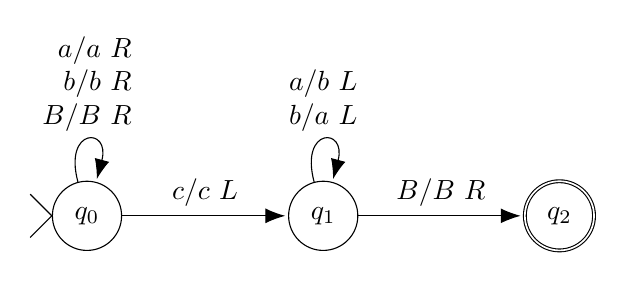
\begin{tikzpicture}[shorten >= 1pt, node distance = 3cm, auto]
            \node[state] (q0) {$q_0$}; %starting node
            \draw (q0.west) -- ++(-3mm,3mm);
            \draw (q0.west) -- ++(-3mm,-3mm);
            \node[state] (q1) [right of=q0] {$q_1$};
            \node[state, accepting] (q2) [right of=q1] {$q_2$};
            
            \path[->]
            (q0) edge [loop above] node[align=right] {$a/a\text{ }R$ \\ $b/b\text{ }R$ \\ $B/B\text{ }R$} (q0)
            (q0) edge node {$c/c\text{ }L$} (q1)
            (q1) edge [loop above] node[align=left] {$a/b\text{ }L$ \\ $b/a \text{ } L$} (q1)
            (q1) edge node {$B/B \text{ }R$} (q2);
          \end{tikzpicture}
        \end{center}
    \end{enumerate}
    This Turing machine, upon reading $c$, replaces every $a$ with $b$ and vice versa before the first $c$ and halts when finished (i.e. upon reading a blank). If there is not at least one $c$, the machine will never halt and thus it will be an infinite computation.
\newpage
  \item Construct a Turing machine with input alphabet $\{a,b,c\}$ that accepts strings in which the first $c$ is immediately preceded by the substring $aaa$. A string must contain a $c$ to be accepted by the machine. \\ \\
    Let this Turing machine be defined by transition table
    \begin{center}
      \begin{tabular}{c|cccc}
        $\delta$ & B & $a$ & $b$ & $c$ \\
        \hline
        $q_0$ & ($q_0,B,R$) & ($q_0,a,R$) & ($q_0,b,R$) & ($q_1,c,L$) \\ 
        $q_1$ & - & ($q_2,a,L$) & - & - \\
        $q_2$ & - & ($q_3,a,L$) & - & - \\
        $q_3$ & - & ($q_4,a,L)$ & - & - \\
        $q_4$ & - & - & - & - \\
      \end{tabular}
    \end{center}
    and state diagram
   
    \begin{center}
      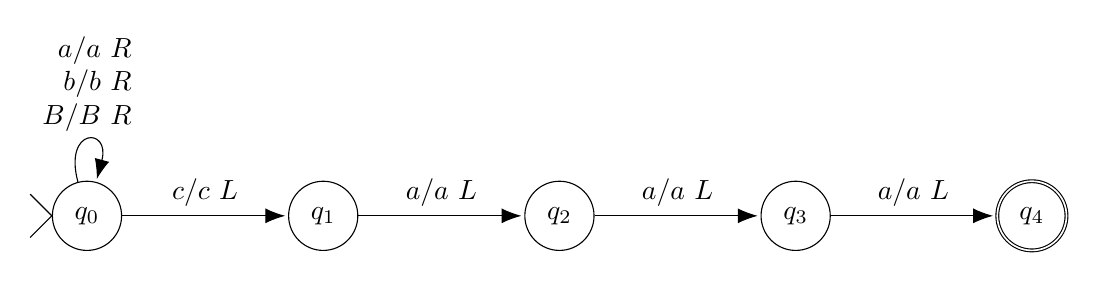
\begin{tikzpicture}[shorten >= 1pt, node distance = 3cm, auto]
        \node[state] (q0) {$q_0$}; %starting node
        \draw (q0.west) -- ++(-3mm,3mm);
        \draw (q0.west) -- ++(-3mm,-3mm);
        \node[state] (q1) [right of=q0] {$q_1$};
        \node[state] (q2) [right of=q1] {$q_2$};
        \node[state] (q3) [right of=q2] {$q_3$};
        \node[state,accepting] (q4) [right of=q3] {$q_4$};        

        \path[->]
        (q0) edge [loop above] node[align=right] {$a/a\text{ }R$ \\ $b/b\text{ }R$ \\ $B/B\text{ }R$} (q0)
        (q0) edge node {$c/c\text{ }L$} (q1)
        (q1) edge node {$a/a\text{ }L$} (q2)
        (q2) edge node {$a/a \text{ } L$} (q3)
        (q3) edge node {$a/a \text{ } L$} (q4);
      \end{tikzpicture}
    \end{center}

\newpage

  \item Construct a Turing machine with input alphabet $\{a,b,c\}$ that accepts the language $L = \{a^ib^ic^i \text{ }|\text{ } i \ge 0\}$ by halting only. \\ \\
    This language is the typical example of a non-context free language, which require matching of three symbols $a,b,$ and $c$ which is beyond the capabilities of regular expressions and even one-stack PDAs to emulate. Turing machines, however, are more than up to the task: By associating each symbol in the language's alphabet with tape alphabet variables $X,Y,$ and $Z$, one can easily keep track of the numbers of each symbol such that they each appear $i$ times. An algorithm for this process is as follows:
    \begin{enumerate}[i.]
    \item Halt on $\lambda$ and accept.
    \item On first $a$, overwrite with $X$, on all other $a$'s and $Y$'s move right. If $b$ go to step (iii), else halt and reject.
    \item On first $b$, overwrite with $Y$, on all other $b$'s and $Z$'s move right. If $c$ go to step (iv), else halt and reject.
    \item On first $c$, overwrite with $Z$, then move left until $X$ is read. 
    \item On $a$, repeat steps (ii-iv). On $Y$, move right on $Y$'s and $Z$'s until $B$ is read, then halt.
    \end{enumerate}
    
    This algorithm can be represented by the following state diagram:
    \begin{center}
      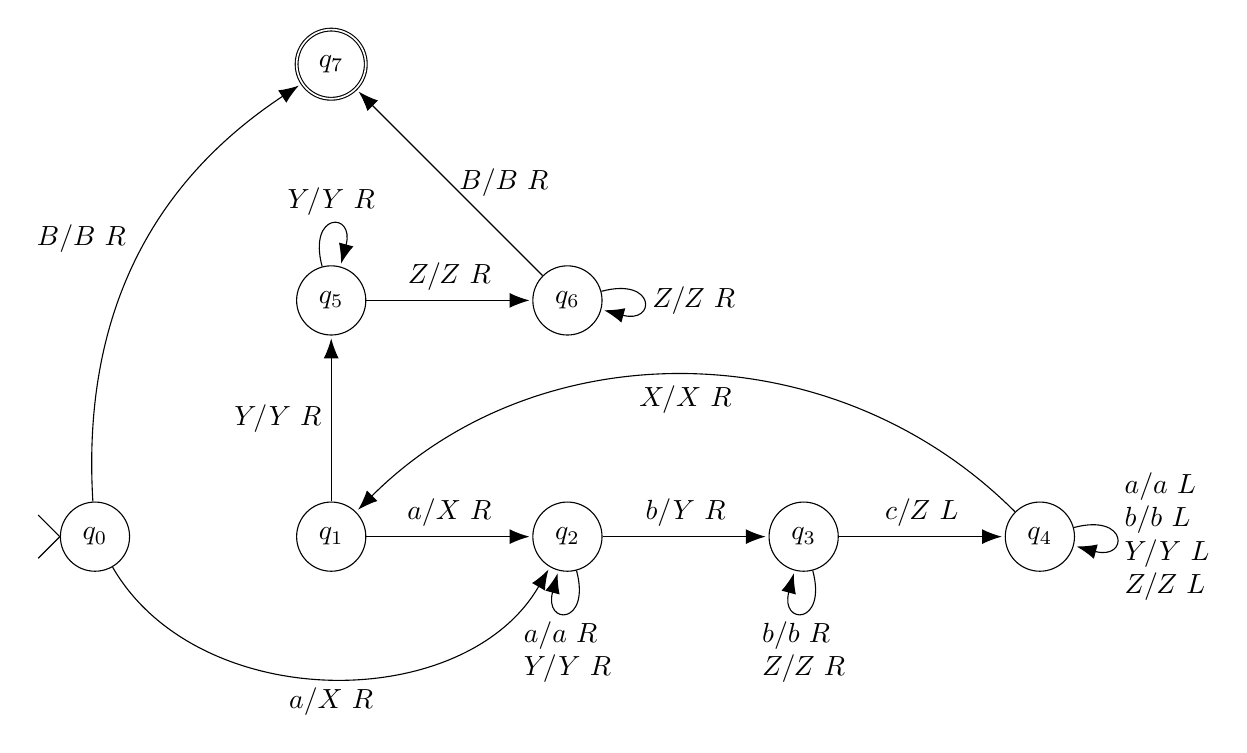
\begin{tikzpicture}[shorten >= 1pt, node distance = 3cm, auto]
        \node[state] (q0) {$q_0$}; %starting node
        \draw (q0.west) -- ++(-3mm,3mm);
        \draw (q0.west) -- ++(-3mm,-3mm);
        \node[state] [right of=q0] (q1) {$q_1$};
        \node[state] [right of=q1] (q2) {$q_2$};
        \node[state] [right of=q2] (q3) {$q_3$};
        \node[state] [right of=q3] (q4) {$q_4$};
        \node[state] [above of=q1] (q5) {$q_5$};
        \node[state] [right of=q5] (q6) {$q_6$};
        \node[state,accepting] [above of=q5] (q7) {$q_7$};
        
        \path[->] 
        (q0) edge [bend right=60] node[below] {$a/X\text{ }R$} (q2)
        (q0) edge [bend left] node {$B/B\text{ }R$} (q7)
        (q1) edge node {$a/X\text{ }R$} (q2)
        (q1) edge node {$Y/Y\text{ }R$} (q5)
        (q2) edge node {$b/Y\text{ }R$} (q3)
        (q2) edge [loop below] node[align=left] {$a/a\text{ }R$ \\ $Y/Y\text{ }R$} (q2)
        (q3) edge node {$c/Z\text{ }L$} (q4)
        (q3) edge [loop below] node[align=left] {$b/b\text{ }R$ \\ $Z/Z\text{ }R$} (q3)
        (q4) edge [bend right=45] node {$X/X\text{ }R$} (q1)
        (q4) edge [loop right] node[align=left] {$a/a\text{ }L$ \\ $b/b\text{ }L$ \\ $Y/Y\text{ }L$ \\ $Z/Z\text{ }L$} (q4)
        (q5) edge [loop above] node {$Y/Y\text{ }R$} (q5)
        (q5) edge node {$Z/Z\text{ }R$} (q6)
        (q6) edge [loop right] node {$Z/Z\text{ }R$} (q6)
        (q6) edge node[right] {$B/B\text{ }R$} (q7);
      \end{tikzpicture}
    \end{center}
  
\newpage

  \item Construct a standard Turing machine that accepts the set of palindromes over $\{a,b\}$. \\ \\
    An even-length palindrome will be of the form $ww^R$, and an odd one of the form $w(a \cup b)w^R$. In both cases, a Turing machine is going to need to match each symbol of $w$ with its corresponding symbol in $w^R$. One algorithm for this is as follows:
    \begin{enumerate}[i.]
    \item If $\lambda$, halt and accept.
    \item If $a$, overwrite with $B$ and remember that starting symbol was $a$. Move right through entire input tape until $B$ is read. Upon reading $B$, read left. If $a$, overwrite with $B$ and move left through entire input tape until $B$ is read, then read right. Else halt and reject.
    \item If $b$, overwrite with $B$ and remember that starting symbol was $b$. Move right through entire input tape until $B$ is read. Upon reading $B$, read left. If $b$, overwrite with $B$ and move left through entire input tape until $B$ is read, then read right. Else halt and reject.
    \item Repeat steps (ii) and (iii) until machine halts. If input tape consists of only blanks, or a single $a$ or single $b$, accept. Else reject.
    \end{enumerate}
This algorithm can be represented with the following state diagram:
    \begin{center}
      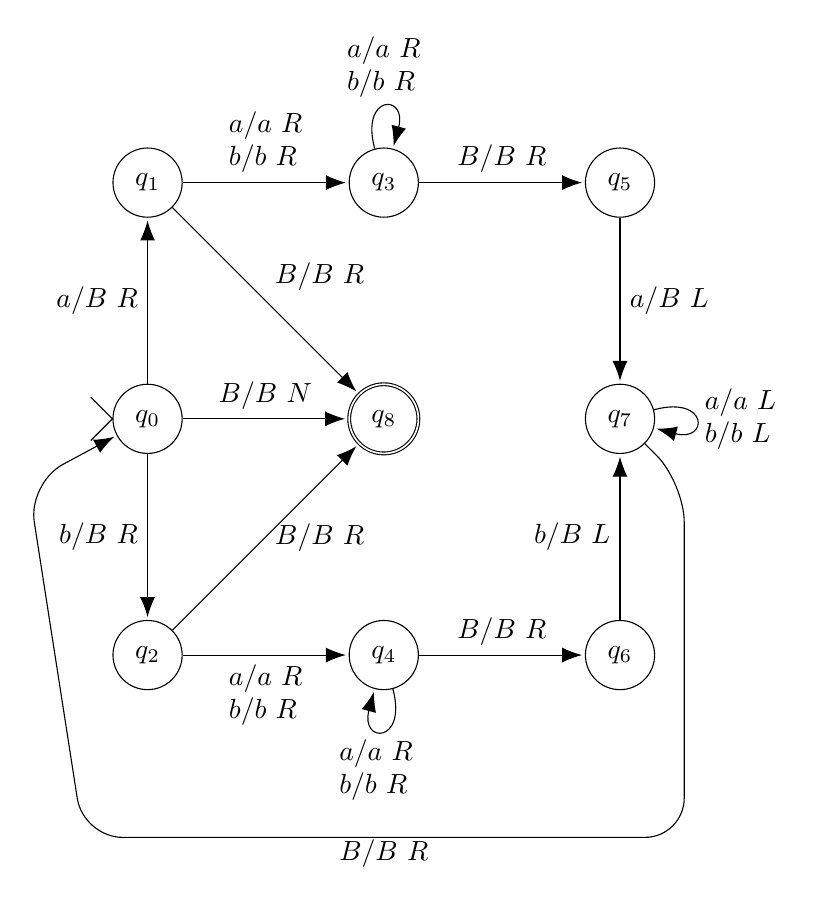
\begin{tikzpicture}[shorten >= 1pt, node distance = 3cm, auto]
        \node[state] (q0) {$q_0$}; %starting node
        \draw (q0.west) -- ++(-3mm,3mm);
        \draw (q0.west) -- ++(-3mm,-3mm);
        \node[state, accepting] (q8) [right of=q0] {$q_8$};
        \node[state] (q1) [above of=q0] {$q_1$};
        \node[state] (q2) [below of=q0] {$q_2$};
        \node[state] (q3) [right of=q1] {$q_3$};
        \node[state] (q4) [right of=q2] {$q_4$};
        \node[state] (q5) [right of=q3] {$q_5$};
        \node[state] (q6) [right of=q4] {$q_6$};
        \node[state] (q7) [right of=q8] {$q_7$};

        \path[->]
        (q0) edge node {$B/B\text{ }N$} (q8)
        (q0) edge node {$a/B\text{ }R$} (q1)
        (q0) edge node[left] {$b/B\text{ }R$} (q2)
        (q1) edge node {$B/B\text{ }R$} (q8)
        (q1) edge node[align=left] {$a/a\text{ }R$ \\$b/b\text{ }R$} (q3)
        (q2) edge node[right] {$B/B\text{ }R$} (q8)
        (q2) edge node[align=left,below] {$a/a\text{ }R$ \\$b/b\text{ }R$} (q4)
        (q3) edge [loop above] node[align=left] {$a/a\text{ }R$ \\$b/b\text{ }R$} (q3)
        (q3) edge node {$B/B\text{ }R$} (q5)
        (q4) edge [loop below] node [align=left] {$a/a\text{ }R$ \\$b/b\text{ }R$ \\ \\ $B/B\text{ }R$} (q4)
        (q4) edge node {$B/B\text{ }R$} (q6)
        (q5) edge node {$a/B\text{ }L$} (q7)
        (q6) edge node {$b/B\text{ }L$} (q7)
        (q7) edge [loop right] node[align=left] {$a/a\text{ }L$ \\$b/b\text{ }L$} (q7);

        \draw[->, rounded corners=5mm] (q7) -- ($(q7.-45) + (0.5,-0.5)$) -- ($(q6.-45) + (0.5,-2)$) -- ($(q2.-135) + (-0.5,-2)$) -- ($(q0.-135) + (-1.2,-0.5)$) -- (q0); % use controls to get huge edge
      \end{tikzpicture}
    \end{center}
\end{enumerate}

\end{document}